%---------TODO----------
% 
%
\chapter{Mecánica estadística de equilibrio}
\section{Fundamentos teóricos}
La mecánica estadística estudia propiedades de los sistemas macroscópicos termodinámicos a partir de las leyes dinámicas microscópicas. Suponemos un sistema aislado caracterizado por las variables termodinámicas energía $U$, volumen $V$ y número de partículas $N$. Una cantidad macroscópica de estado (ó {\it macroestado} $(U,V,N)$) en el sistema es el promedio de propiedades microscópicas, en cambio, un estado microscópico del sistema está definido por coordenadas $q$ y momentos $p$ correspondientes al macroestado $(U,V,N)$, este se denomina {\it microestado}. El total de microestados asociados a un macroestado se denota por $\Omega(U,V,N)$.\\

% De acuerdo con la mecánica clásica, la dinámica de un sistema de partículas se resuelve solucionando las ecuaciones de movimiento de las partículas.
% Sin embargo, cuando las partículas interactúan entre sí, resolver la dinámica del sistema por cualquiera de los métodos en dinámica (Newton, Lagrange o Hamilton) sería un cálculo básicamente imposible o poco práctico. A pesar de ello el marco conceptual es extremadamente útil y por ello describiremos enseguida los postulados de la mecánica estadística de equilibrio y el concepto de ensamble.\\

Dos postulados fundamentales de la física estadística crean dicha conexión entre las escalas microscópica y macroscópica:\\

\begin{itemize}
    \item Postulado de equiprobabilidad: Cuando un sistema macroscópico está en equilibrio termodinámico, sus microestados asociados son igualmente probables \cite{Huang_1987}.\\
    
    \item Postulado de la entropía: En un sistema en equilibrio, su entropía $S$ está dada por \cite{tuckerman2010}:
    \begin{equation}\label{postulado_entropia_boltx}
        S=Kln(\Omega)
    \end{equation}
    con K una constante y $\Omega$ el número de microestados correspondientes.
\end{itemize}


\section{Ensambles}

Un ensamble es una colección hipotética de $N$ réplicas descritas por el mismo conjunto de interacciones microscópicas y que comparten un conjunto de propiedades macroscópicas (Energía, volumen, número de partículas, etc.) \cite{tuckerman2010}.\\

% Los ensambles pueden ser definidos dependiendo de las situaciones termodinámicas que se impongan al sistema, y dependiendo de \textcolor{yellow}{estos} se pueden extraer propiedades estáticas macroscópicas como la energía, temperatura, presión, etc. Los ensambles que cumplen esta propiedad estática aun cuando el sistema se encuentra evolucionando en el tiempo son llamados \textit{Ensambles de equilibrio}.\\
En teoría clásica de ensambles todas las observables macroscópicas de un sistema están conectados a una función microscópica. 

Se puede calcular el promedio temporal de una variable dinámica $A$ como en la ecuación (\ref{promediotemp}), 

\begin{equation} \label{promediotemp}
    \langle A\rangle_{tiempo} = \lim_{t\to\infty}\frac{1}{t}\int_0^t A(t)dt
\end{equation}\\
en el intervalo de tiempo de 0 a $t$,
o por un promedio de ensamble asociado a su probabilidad como en la ecuación (\ref{promedioequprob}) \cite{tuckerman2010}. \\
\begin{equation} \label{promedioequprob}
    \langle A\rangle_{ensamble} =\sum_r A_r P_r
\end{equation}\\
con $P_r$ la probabilidad del r-ésimo microestado y $A_r$ el valor de $A$ en el r-ésimo microestado.\\

Las ecuaciones (\ref{promediotemp}) y (\ref{promedioequprob}) se encuentran directamente relacionados por dos enunciados importantes:

\begin{itemize}
    \item Postulado de Gibbs: El promedio de una propiedad mecánica corresponde a un propiedad termodinámica paralela \cite{mcquarrie1976}.\\
    
    \begin{equation}
        E \Longleftrightarrow \left \langle E \right \rangle
    \end{equation}
    
    \item Hipótesis ergódico: Medir un sistema para N instantes en el tiempo tiene las mismas propiedades estadísticas que medir N sistemas arbitrarios al mismo tiempo de un ensamble \cite{mcquarrie1976}:
    \begin{equation}
        \left \langle A \right \rangle_{tiempo} \Longleftrightarrow \left \langle A \right \rangle_{ensamble}
    \end{equation}
\end{itemize}


La Tabla \ref{tiposEnsamble} resume cuatro de los ensambles de equilibrio más comúnmente usados.

\begin{table}[h!]
    \centering
    \begin{tabular}{ |p{1cm}||p{4cm}|  }
    \hline
    \multicolumn{2}{|c|}{Ensambles} \\
    \hline
    NVE   & Microcanónico \\
    NVT   & Canónico \\
    $\mu$VT& Gran Canónico \\
    NPT   & Isotérmico-Isobárico \\
    \hline
    \end{tabular}
    \caption{Tipos de Ensambles}
    \label{tiposEnsamble}
\end{table}

\subsection{Ensamble Canónico NVT}

El ensamble canónico está formado por $\mathcal{N}$ copias de un sistema en equilibrio con N partículas, una fuente de calor a temperatura T. Los $\mathcal{N}$ sistemas del ensamble están en contacto entre si mediante paredes diatérmicas, es decir, para cada sistema en este ensamble, el resto es su fuente de calor como se muestra en la figura \ref{fig:CanonicEns}.\\

\begin{figure}[!h]
    \centering
    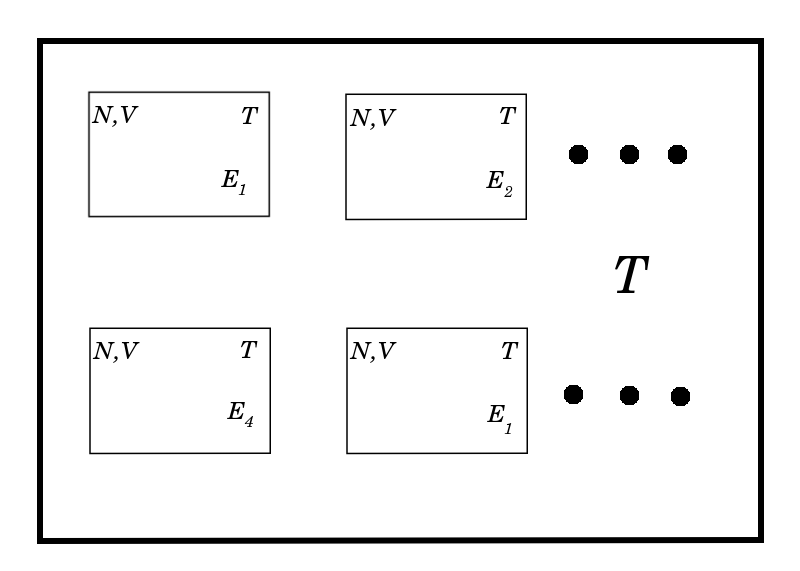
\includegraphics[width=.55\textwidth,keepaspectratio=true]{EnsCanonico.png}
    \caption{Representación del ensamble canónico NVT \cite{belof2013alternative}}
    \label{fig:CanonicEns}
\end{figure}

\newpage

Los sistemas del ensamble se encuentran en algunos de los $E_r$ niveles de energía, estos a su vez toman y ceden energía con su alrededor, es decir, los otro sistemas. Puede haber degeneración en algunos sistemas (sistemas diferentes pueden tener el mismo nivel de energía macroscópico).\\

De acuerdo a lo anterior, tenemos:\\
\begin{center}
    $N_1$ sistemas con energía $E_1$\\
    $N_2$ sistemas con energía $E_2$\\
    ...\\
    $N_r$ sistemas con energía $E_r$\\
    ...\\
\end{center}


Lo previo cumple las ecuaciones (\ref{restrprob}) y (\ref{energiaprob}):

\begin{equation} \label{restrprob}
    1 = \sum_r P_r \\
\end{equation}

\begin{equation} \label{energiaprob}
    \langle E\rangle = \sum_r P_r E_r
\end{equation}

\begin{center}
    con $P_r = \frac{N_r}{\mathcal{N}}$
\end{center}


El número de formas de microestados correspondientes en que se presenta esta distribución es:\\ \textcolor{red}{Dar una mejor explicación}

\begin{equation} \label{ditrbmicro}
    \Omega = \frac{\mathcal{N}!}{\prod_r N_r}
\end{equation}\\

Por la ecuación (\ref{postulado_entropia_boltx}) y de acuerdo con la fórmula de Stirling se encuentra la ecuación (\ref{entropiaboltz})

\begin{equation}  \label{entropiaboltz}
    S = Kln(\frac{\mathcal{N}}{\prod_r N_r}) = -K\mathcal{N}\sum_r P_rln(P_r)
\end{equation}\\

Aplicando el método de los multiplicadores de Lagrange se halla lo siguiente \cite{greiner1995}:

\begin{equation} \label{probcan}
    P_r = \frac{e^{-\beta E_r}}{\mathcal{Z}}
\end{equation}
\begin{equation*} \label{funcpartcan}
    \text{donde }\mathcal{Z} = \sum_r e^{-\beta E_r \quad con\ \beta=\frac{1}{KT}} \text{ es la función de partición canónica}
\end{equation*}


Así, la entropía dentro de unos de los sistemas del ensamble es \cite{mandl1988statistical}:

\begin{equation} \label{entrnvt}
    S = K\beta U + Kln(\mathcal{Z})
\end{equation}

Todas las propiedades termodinámicas se obtienen de la función de partición canónica como se muestra en las ecuaciones (\ref{energcan}) (\ref{ecestacan}).

\begin{equation} \label{energcan}
    U=-\frac{\partial}{\partial \beta}ln(\mathcal{Z})
\end{equation}

\begin{equation} \label{ecestacan}
    PV=KTln(\mathcal{Z})
\end{equation}

El potencial termodinámico del ensamble canónico es la energía libre de Helmholtz:

\begin{equation} \label{potHelm}
    F(N,V,T)=-\frac{1}{\beta}ln(\mathcal{Z})=U-TS
\end{equation}

\subsection{Ensamble isotérmico-isobárico NPT}

El ensamble NPT esta formado por $\mathcal{N}$ copias de un sistema en equilibrio con N partículas, una fuente de calor a temperatura T y esta acoplado a un pistón isotrópico que se comprime o expande en respuesta a fluctuaciones instantáneas de la presión interna (fuente de volumen). Los $\mathcal{N}$ sistemas de este ensamble estan en contacto entre si por paredes diatérmicas y flexibles, es decir, para cada sistema en este ensamble, el resto es su fuente de calor y de volumen como se muestra en la figura \ref{fig:NPTEns}.\\

Este ensamble es importante porque los datos experimentales de propiedades en fase condensada se encuentran a condiciones de presión y temperatura constante.\\


\begin{figure}[!h]
    \centering
    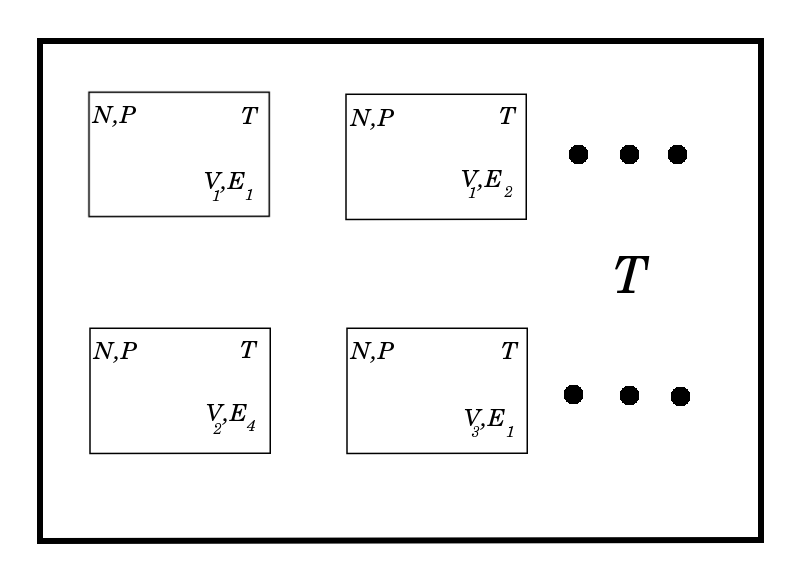
\includegraphics[width=.55\textwidth,keepaspectratio=true]{nptensemble.png}
    \caption{Representación del ensamble NPT \cite{belof2013alternative}}
    \label{fig:NPTEns}
\end{figure}

\newpage

Tenemos en este sistema lo siguiente:\\

\begin{center}
    $N_{1n}$ sistemas con energía $E_{1n}$ y volumen $V_1$\\
    $N_{2n}$ sistemas con energía $E_{2n}$ y volumen $V_2$\\
    ...\\
    $N_{rn}$ sistemas con energía $E_{rn}$ y volumen $V_r$\\
    ...\\
\end{center}

Lo anterior debe cumplir con las ecuaciones (\ref{restrprobNPT})-(\ref{volprobNPT}).

\begin{equation} \label{restrprobNPT}
    1 = \sum_r P_r \\
\end{equation}

\begin{equation} \label{energiaprobNPT}
    U = \langle E\rangle = \sum_{rn} P_{rn} E_{rn}
\end{equation}

\begin{equation} \label{volprobNPT}
    V = \langle E\rangle = \sum_{rn} P_{rn} V_r
\end{equation}

\begin{center}
    con $P_{rn} = \frac{N_{rn}}{\mathcal{N}}$
\end{center}

El número de formas de microestados correspondientes en que se presenta esta distribución es:\\ \textcolor{red}{Referir a la explicación que dé en el ensamble anterior}

\begin{equation} \label{distribucionmultnom}
    \Omega = \frac{\mathcal{N}!}{\prod_{rn} N_{rn}}
\end{equation}\\

Por el postulado de la entropía y de acuerdo a la formula de Stirling obtenemos la siguiente ecuación:

\begin{equation}  \label{entropiaboltzNPT}
    S = kln(\frac{\mathcal{N}}{\prod_{rn} N_{rn}}) = -K\mathcal{N}\sum_{rn} P_{rn} ln(P_{rn})
\end{equation}\\

Usando el método de los multiplicadores de Lagrange se encuentra la siguiente ecuación:

\begin{equation} \label{probNPT}
    P_{rn} = \frac{e^{-\beta E_{rn}-\xi V_r}}{\mathcal{Z}}
\end{equation}
\begin{equation*} \label{funcpartNPT}
    \text{donde }\mathcal{Z} = \sum_{rn} e^{-\beta E_{rn}-\xi V_r} \quad con\ \beta=\frac{1}{KT} \quad y\ \xi=\frac{P}{KT}\text{ es la función de partición}
\end{equation*}

La entropía de uno de los sistemas del ensamble es \cite{mcquarrie1976}:

\begin{equation} \label{entrpnpt}
    S = k\beta U + k\xi V + kln(\mathcal{Z})
\end{equation}

Todas las propiedades termodinámicas se obtienen de la función de partición encontrada como se muestra en las ecuaciones (\ref{energNPT})-(\ref{ecestaNPT}).

\begin{equation} \label{energNPT}
    U=-\frac{\partial}{\partial \beta}ln(\mathcal{Z})
\end{equation}

\begin{equation} \label{volNPT}
    V=-\frac{\partial}{\partial \xi}ln(\mathcal{Z})
\end{equation}

\begin{equation} \label{ecestaNPT}
    PV=KTln(\mathcal{Z})
\end{equation}

El potencial termodinámico del ensamble isotérmico-isobárico es la energía libre de Gibbs \cite{mcquarrie1976}:

\begin{equation} \label{potgibbs}
    G(N,P,T)=-\frac{1}{\beta}ln(\mathcal{Z})=U-TS+PV
\end{equation}\\

\section{Mecánica estadística clásica de N partículas interactuantes} \label{MecClasNpart}

\textcolor{blue}{
Las aplicaciones de la mecánica estadística más inmediatas se realizan en sistemas donde las partículas no interactúan entre sí y corresponden a los casos \textit{ideales}. En estos sistemas los cálculos son analíticos y generalmente existe una solución exacta al problema del cálculo de la función de partición o de las propiedades del sistema. Sin embargo, esta aproximación no siempre es razonable, en particular en sistemas densos donde las partículas interactúan y generan el estado líquido de una sustancia. En estas condiciones la moléculas y átomos interactúan para crear lo que conocemos como el estado líquido del agua y cuyas propiedades experimentales no pueden ser descritas considerando al sistema como ideal.}\\

Supongamos un fluido con $N$ partículas que interactúan a través de un potencial conservativo $\mathcal{V}$. En el formalismo lagrangiano las ecuaciones de movimiento son (\ref{lagrangeeq}) \cite{torresdelcastillo_2018}\\

\begin{equation} \label{lagrangeeq}
    \frac{d}{dt}\frac{\partial L}{\partial \dot r_i} - \frac{\partial L}{\partial r_i} = 0,
\end{equation}\\
donde $L$ es el lagrangiano del sistema como se muestra en (\ref{lagrangiano})

\begin{equation} \label{lagrangiano}
    L = \sum_{i=1}^{N} \frac{1}{2}m_i\dot{\vec{r_i}}^2-\mathcal{V}({\vec{r}}_1,{\vec{r}}_2,...,{\vec{r}}_N).
\end{equation}\\
El potencial $\mathcal{V}$ caracteriza la interacción entre moléculas en el sistema \cite{torresdelcastillo_2018} y la fuerza sobre la partícula $i$ se obtiene a través de

\begin{equation}
    F_i({\vec{r}}_1,{\vec{r}}_2,...,{\vec{r}}_N) = -\nabla_{r_i}\mathcal{V}({\vec{r}}_1,{\vec{r}}_2,...,{\vec{r}}_N).
\end{equation}\\

Adicionalmente, para el lagrangiano $L$ de la ecuación \ref{lagrangiano}, el hamiltoniano clásico es igual a la energía y están dados por

\begin{equation} \label{hamiltoniano}
    H(\vec{p},\vec{q}) = E = \sum_{i=1}^{N} \frac{1}{2 m_i}\vec{p_i}^2 + \sum_{i=1}^{N-1}\sum_{j=i+1}^{N} u(r_{ij})
\end{equation}\\

donde $u(r_{ij})$ es una energía potencial entre pares que depende únicamente de la distancia entre estas y $\vec{p_i}$ es el momento lineal que se denota por (\ref{momlin}).

\begin{equation}\label{momlin}
    \vec{p_i} = m\dot{\vec{r_i}}
\end{equation}

En el límite termodinámico las sumas en las funciones de partición se vuelven integrales en el espacio fase. Para un sistema con partículas clásicas independientes e indistinguibles, la función de partición en coordenadas cartesianas es \cite{mcquarrie1976},

\begin{equation} \label{funcpartclas}
    \mathcal{Z} = \frac{1}{N!h^{3N}}\int ...\int e^{-\beta H(\vec{r},\vec{p})}dx_1dy_1dz_1dp_{x_1}dp_{y_1}...dy_N dz_Ndp_{x_N}dp_{y_N}dp_{z_N}.
\end{equation}\\

Sustituyendo la ecuación (\ref{hamiltoniano}) en la ecuación (\ref{funcpartclas}) \cite{feynman1972statistical}:

\begin{equation} \label{funcpartclasconfig}
    \mathcal{Z} = \frac{1}{N!}\left( \frac{2\pi m}{\beta h^2} \right)^{3N/2}Z_N,\quad con\ Z_N = \int e^{-\beta \mathcal{V}}dx_1dy_1dz_1...dx_N dy_N dz_N
\end{equation}\\

donde $Z_N$ es la integral de configuración clásica.

\textcolor{green}{Sugiero que la siguiente sección se titule 
Interacciones intermoleculares y se agregue una breve descripción de interacciones de Van der Waals y de interacción de Coulomb, posteriormente ya puedes mencionar que el potencial de Lennard-Jones modela a las primeras y a interacciones repulsivas de corto alcance}


\section{Interacciones intermoleculares}

Las interacciones de Van der waals son interacciones atractivas causadas por las nubes electrónicas de los átomos cuando están a distancias del orden de angstroms, sin embargo, se repelen fuertemente cuando se encuentran extremadamente cerca para evitar traslapes de nubes electrónicas (exclusión de pauli).\\

Estas interacciones dependen de la distancia a la 6ta potencia y son débiles enérgicamente en comparación con la energía cinética de una molécula en una solución \cite{201753}. La fuerza de Van der waals tiene tres variantes \cite{ROY20151}: \textcolor{red}{Checar citas aquí ya que no coinciden con la información que informo} \textcolor{blue}{En la página 11 se presenta un resumen de una página sobre las tres fuerzas y la interacción de van der waals}

\begin{itemize}
    \item Fuerza Keesom: Fuerza de atracción entre dos dipolos permanentes.
    \item Fuerza Debye: Fuerza de atracción entre un dipolos permanentes y un dipolo inducido.
    \item Fuerza London: Fuerza de atracción entre dos dipolos inducidos.
\end{itemize}

La interacción o fuerza de coulomb es la mas fuerte en las interacciones intermoleculares y a veces tan fuerte como los enlaces químicos, la fuerza depende inversamente del cuadrado de la distancia como se puede observar en la ecuación (\ref{coulombforce}) \cite{ISRAELACHVILI201153}.

\begin{equation} \label{coulombforce}
    F(r_{ij}) = \frac{q_i q_j}{4\pi \epsilon r^2_{ij}}
\end{equation}

\subsection{Potencial de Lennard-Jones}

El potencial de Lennard-Jones 12-6 es:

\begin{equation} \label{LJ12-6}
    v^{LJ} = 4\epsilon \left[ \left(\frac{\sigma}{r} \right)^{12}-\left(\frac{\sigma}{r} \right)^{6}\right]
\end{equation}\\

$r:= |\vec{r_1}-\vec{r_2}|$\\

$\sigma: $ valor de r donde $v^{LJ}(r)=0$\\

$\epsilon : $profundidad del pozo del potencial\\

Este potencial entre pares modela interacciones atractivas de Van der Waals y a las repulsivas de corto alcance. Es usado de manera frecuente en los campos de fuerza los cuales se mencionan mas adelante en el texto. Los valores de $\sigma$ y $\epsilon$ se ajustan a propiedades conocidas del átomo en cuestión. A continuación en la figura \ref{fig:LJ126} se muestra un potencial Lennard-Jones 12-6:\\

\begin{figure}[!h]
    \centering
    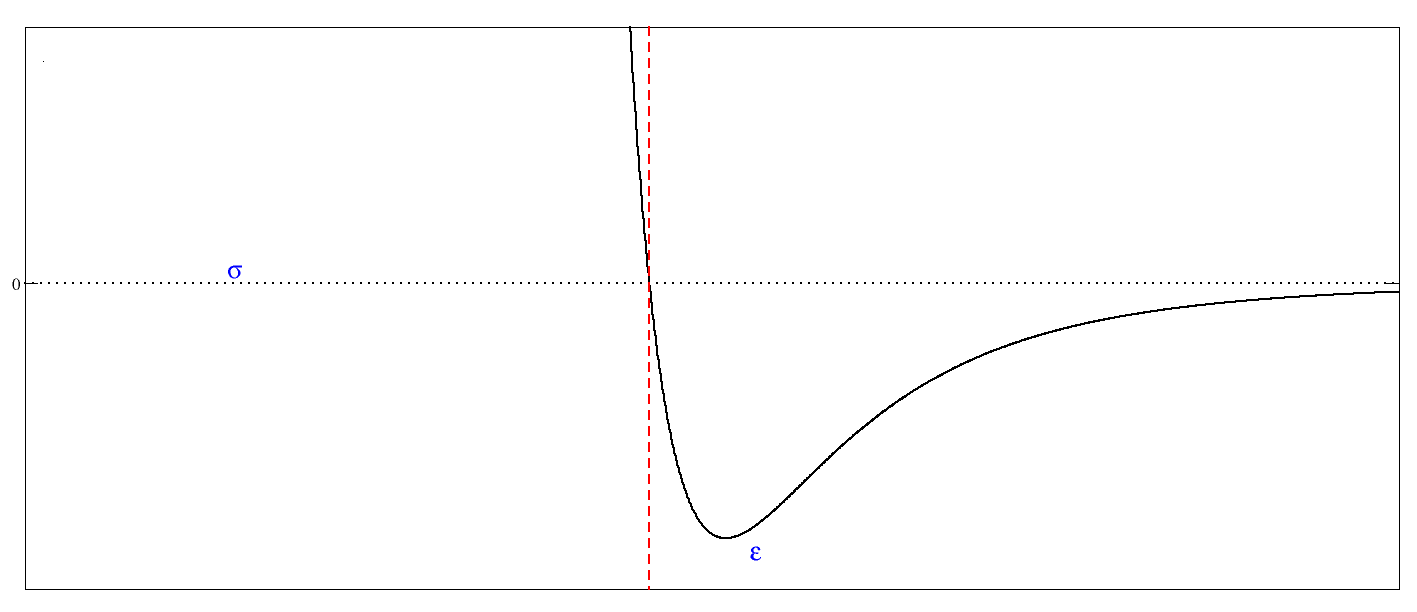
\includegraphics[width=1\textwidth,keepaspectratio=true]{LJ.png}
    \caption{Potencial Lennard-Jones}
    \label{fig:LJ126}
\end{figure}

Este potencial esta dividido en tres intervalos en el eje $r$ \cite{ADAMS2001763}:

\begin{itemize}
    \item El primer intervalo es el potencial repulsivo que está antes de la linea roja en la figura \ref{fig:LJ126}, este es para evitar el traslape de nubes electrónicas (Principio de exclusión de pauli).
    \item El pozo del potencial es debido a la cohesión en la fase condensada de la materia.
    \item La parte atractiva de este potencial es causada por la interacción de van der waals.
\end{itemize}

\begingroup
\let\clearpage\relax
\chapter{Nanotubos de carbono}
\endgroup

\section{Estructura de los nanotubos de carbono}

% En la simulación presentada se usó un nanotubo de carbono de una capa (SWCNT por sus siglas en ingles), por lo que es necesario explicar características, geometría y algunas propiedades de estos nanomateriales.\\
Los nanotubos de carbonos son una sabana de un arreglo hexagonal de carbono enrollados en un eje para formar un cilindro, fueron descubiertos por Iijima en experimentos usando el método de arco de descarga en 1991 \cite{Iijima1991}.\\

\begin{table}[h!]
    \centering
    \begin{tabular}{ |p{2cm}|p{3cm}|  }
    \hline
    \multicolumn{2}{|c|}{Características} \\
    \hline
    $a_{cc}$   & 1.42 \AA \\
    \hline
    C-C-C($\theta$)   & 120 $\deg$ \\
    \hline
    q & 0e \\
    \hline
    m   & 12.0107 u \\
    \hline
    \end{tabular}
    \caption{Caracteristicas del carbono y enlaces de carbono \cite{Melendez2016}}
    \label{carbono}
\end{table}


\section{Geometría y notación (n,m)}

\begin{figure}[!h] 
    \centering
    \begin{minipage}{0.45\textwidth}
    \centering
    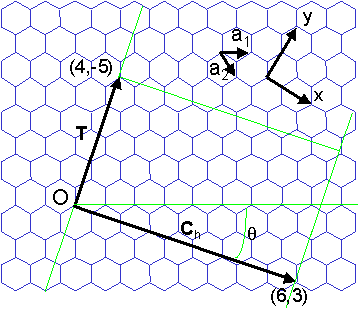
\includegraphics[width=0.95\textwidth]{ChCNT.png}
    \end{minipage}
    \begin{minipage}{0.45\textwidth}
    \centering
    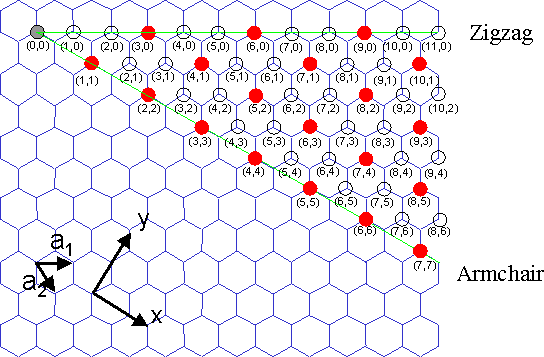
\includegraphics[width=1.2\textwidth]{NT.png}
    \end{minipage}
    \caption{Chiralidad y simetría en nanotubos \cite{ShigeoChiral}}
\end{figure} \label{fig:GeoVectChir}

La geometría se puede describir usando los vectores $\vec{a_1}$ y $\vec{a_2}$ por convención están arreglados como se muestra en las figuras [2.1]. Usando estos podemos describir las siguientes características \cite{Melendez2016}:\\

\begin{itemize}
    \item Vector quiral (n,m): $C_h = n\vec{a_1} + m\vec{a_2}$
    \item Magnitud del vector quiral: $\left|C_h\right| = \sqrt{3}a_{cc}\sqrt{n^2+m^2+nm}$
    \item Diámetro del nanotubo: $d_T = \left|C_h\right|/\pi$
\end{itemize}

El vector de traslación $\vec{T}$ es el vector más corto perpendicular a $C_h$ que empieza y termina en un punto del arreglo hexagonal:

\begin{itemize}
    \item Vector de traslación: $\vec{T} = \left[\left(2m+n\right)\vec{a_1} - \left(2n+m\right)\vec{a_2}\right]/d_R$
    \item Magnitud del vector de traslación: $\left|\vec{T}\right|=\sqrt{3}a_{cc}\frac{\left|C_h\right|}{d_R}$
\end{itemize}

donde:

\begin{equation}\label{dR}
    d_R =
    \begin{cases} 
    d,& \text{si } n-m \text{ no es múltiplo de } 3d\\
    3d,& \text{si } n-m \text{ es múltiplo de } 3d
    \end{cases}
\end{equation}\\

Los nanotubos están categorizados por su notación (n,m) \cite{Melendez2016}:

\begin{itemize}
    \item Armchair: (n,n) $\left|C_h\right|=3na_{cc}$ y $\left|\vec{T}\right|=\sqrt{3}a_{cc}$
    \item Zigzag: (n,0) $\left|C_h\right|=\sqrt{3}na_{cc}$ y $\left|\vec{T}\right|=3a_{cc}$
    \item Quiral: (n,m) where 0 < m < n
\end{itemize}

Para un SWCNT (n,m), si n = m el nanotubo es metálico; si n - m es múltiplo de 3, el nanotubo es casi-metálico, de otra manera el nanotubo es un semiconductor. En la figura [2.1] los puntos rojos representan los nanotubos metálicos y los círculos negros representan los semiconductores.\\

Lo anterior asegura que la notación (n,m) define completamente la estructura de un SWCNT.

\begingroup
\let\clearpage\relax
\chapter{Dinámica molecular}
\endgroup

La imposibilidad de hacer cálculos manuales de la mecánica estadística como método para estudiar fluidos interactuantes y con la llegada de la alta capacidad de procesamiento computacional dio lugar a la posibilidad de usar la aproximación Born-Oppenheimer(aproximación para escribir el hamiltoniano en términos de sus interacciones nucleares donde sus movimientos de electrones han sido promediados) para resolver las ecuaciones de movimiento de Newton para sistemas atómicos. \\

La simulación conecta los resultados experimentales con los modelos de simulación y viceversa, mediante las propiedades termodinámicas del sistema. La simulación molecular de un sistema nos permite introducir detalles microscópicos de los átomos y moléculas como geometrías, masas, interacciones entre ellas, etc.\\


\begin{figure}[!h]
    \centering
    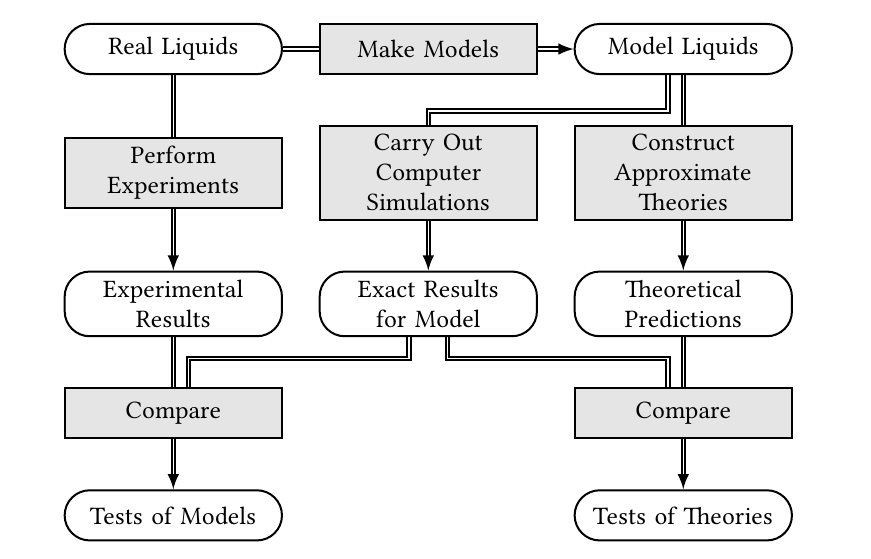
\includegraphics[width=.7\textwidth,keepaspectratio=true]{conexionteoriaexpsim.png}
    \caption{Conexión entre teoría, experimentación y simulación molecular \cite{Allen2017}}
    \label{fig:conteexpsim}
\end{figure}

\section{Fundamentos de dinámica molecular}

La dinámica molecular resuelve las ecuaciones de movimiento descritas en la sección \ref{MecClasNpart} para un sistema atómico, molecular o centros de masa de configuraciones moleculares. Las ecuaciones de hamilton para el hamiltoniano en la ecuación (\ref{hamiltoniano}) son:\\

\begin{equation}
    \mathbf{r}_i = \mathbf{p}_i/m_i \\
\end{equation}\\
\begin{equation}
    \mathbf{\dot p}_i = -\nabla_{\mathbf{r}_i}\mathcal{V} = \mathbf{F}_i
\end{equation}\\

Sin embargo, una ventaja de la convención lagrangiana es la posibilidad de incorporar fuerzas de constricción a las ecuaciones de movimiento de forma directa, donde $g_i$ es la fuerza de constricción \cite{raabe2017}:\\

\begin{equation} \label{lagrangeeqconstraint}
    \frac{d}{dt}\frac{\partial L}{\partial \dot r_i} - \frac{\partial L}{\partial r_i} = g_i
\end{equation}\\

\section{Métodos de diferencia finitas}

La solución de las ecuaciones de movimiento se pueden resolver numéricamente por computadora con métodos de diferencias finitas. Existen diferentes algoritmos que son computacionalmente eficientes.\\

Los algoritmos de integración usados en este trabajo son sencillos de derivar. Primero, se realiza una expansión de McLaurin de la posición, velocidad y aceleración alrededor del paso $\delta t$:

\begin{align} \label{taylorexpr}
\begin{split}
    \mathbf{r}(t + \delta t) &= \mathbf{r}(t)+\delta t\dot{\mathbf{r}}(t) + \frac{1}{2}\delta t^2 \ddot{\mathbf{r}}(t)+...\\
                             &= \mathbf{r}(t)+\delta t\mathbf{v}(t) + \frac{1}{2}\delta t^2 \mathbf{a}(t)+...
\end{split}
\end{align}
\begin{equation}\label{taylorexpv}
    \mathbf{v}(t + \delta t) = \mathbf{v}(t)+\delta t\mathbf{a}(t) + \frac{1}{2}\delta t^2 \mathbf{j}(t)+...
\end{equation}
\begin{equation}\label{taylorexpa}
    \mathbf{a}(t + \delta t) = \mathbf{a}(t)+\delta t\mathbf{j}(t) + \frac{1}{2}\delta t^2 \dot{\mathbf{j}}(t)+...
\end{equation}\\

Las ecuaciones son iterativas, dada la función dinámica anterior a un tiempo $t$ podemos conocer la función en el siguiente paso $t + \delta t$.

\subsection{Algoritmo de Verlet}

Calculamos otras series de McLaurin de $\mathbf{v}(t+\frac{1}{2}\delta t)$ y $\mathbf{r}(t-\delta t)$.\\

\begin{equation}\label{taylorexpr-}
    \mathbf{r}(t - \delta t) = \mathbf{a}(t)+\delta t\mathbf{j}(t) + \frac{1}{2}\delta t^2 \mathbf{\dot{j}}(t)-...
\end{equation}

La ecuación (\ref{verletv1/2}) es la primera ecuación de Verlet:\\
\begin{equation}\label{verletv1/2}
    \mathbf{v}(t + \frac{1}{2}\delta t) = \mathbf{v}(t)+\frac{1}{2}\delta t\mathbf{a}(t) +...
\end{equation}\\

Sustituyendo la ecuación (\ref{verletv1/2}) en la ecuación (\ref{taylorexpr}) obtenemos la segunda ecuación de Verlet:

\begin{align} \label{verletr}
\begin{split}
    \mathbf{r}(t + \delta t) &= \mathbf{r}(t)+\delta t\dot{\mathbf{r}}(t) + \frac{1}{2}\delta t^2 \ddot{\mathbf{r}}(t)+...\\
                             &= \mathbf{r}(t)+\delta t\left[\mathbf{v}(t) + \frac{1}{2}\delta t \mathbf{a}(t)+...\right]\\
                             &= \mathbf{r}(t)+\delta t \mathbf{v}(t+\frac{1}{2}\delta t)
\end{split}
\end{align}

Sustituyendo las ecuaciones (\ref{verletv1/2}) y (\ref{taylorexpa}) en la ecuación (\ref{taylorexpv}) obtenemos la tercera ecuación de verlet:

\begin{align} \label{verletv}
\begin{split}
    \mathbf{v}(t + \delta t) &= \mathbf{v}(t)+\delta t\mathbf{a}(t) + \frac{1}{2}\delta t^2 \mathbf{j}(t)+...\\
                             &= \mathbf{v}(t)+\frac{1}{2}\delta t\mathbf{a}(t) + \frac{1}{2}\delta t\mathbf{a}(t)+ \frac{1}{2}\delta t^2 \mathbf{j}(t)+...\\
                             &= \mathbf{v}(t + \frac{1}{2}\delta t) + \frac{1}{2}\delta t\mathbf{a}(t + \delta t)
\end{split}
\end{align}

Pasos del algoritmo:

\begin{enumerate}
    \item Calcular la ecuación (\ref{verletv1/2}).
    \item Con el resultado del paso anterior, calcular la ecuación (\ref{verletr}).
    \item Computar las fuerzas sobre la partícula para obtener la aceleración en $t + \delta t$.
    \item $t = t + \delta t$
    \item Regresamos al primer paso
\end{enumerate}

También si se quiere obtener la energía cinética se deriva la siguiente formula de la velocidad usando (\ref{taylorexpv}) y (\ref{taylorexpr-}):

\begin{equation}
    \mathbf{v}(t)=\frac{\mathbf{a}(t + \delta t)-\mathbf{r}(t - \delta t)}{2\delta t}
\end{equation}

\subsection{Algoritmo salto de rana(leap frog scheme)}

Otra alternativa del algoritmo de Verlet es \cite{Allen2017}:\\

\begin{equation} \label{leapfrogv1/2}
    \mathbf{v}(t + \frac{1}{2}\delta t)=\mathbf{v}(t - \frac{1}{2}\delta t)+\delta t\mathbf{a}(t)
\end{equation}

\begin{equation} \label{leapfrogr}
    \mathbf{r}(t + \delta t)= \mathbf{r}(t)+\delta t \mathbf{v}(t+\frac{1}{2}\delta t)
\end{equation}

\textcolor{red}{Agregar pasos del algoritmo de salto de rana bien expicados}

\begin{enumerate}
    \item Calcular la ecuación (\ref{verletv1/2}).
    \item Con el resultado del paso anterior, calcular la ecuación (\ref{verletr}).
    \item Computar las fuerzas sobre la partícula para obtener la aceleración en $t + \delta t$.
    \item $t = t + \delta t$
    \item Regresamos al primer paso
\end{enumerate}

Se almacena en memoria $\mathbf{r}(t)$, $\mathbf{v}(t - \frac{1}{2}\delta t)$ y computamos fuerzas para obtener $\mathbf{a}(t)$, con estos resultados en memoria podemos empezar calculando la ecuación (\ref{leapfrogv1/2}) para usarlo en la ecuación (\ref{leapfrogr}).

\section{Condiciones de frontera periódicas y convención de minima imagen}

Supongamos un cubo de simulación de longitud L, si se deseara realizar una simulación del sistema se necesitaría establecer la interacción molécula-pared. Para evitar estas interacciones empleamos condiciones de frontera periódicas: cuando una partícula deja el cubo, su imagen entra por la cara opuesta como en la figura \ref{fig:PBC}

\begin{figure}[!h]
    \centering
    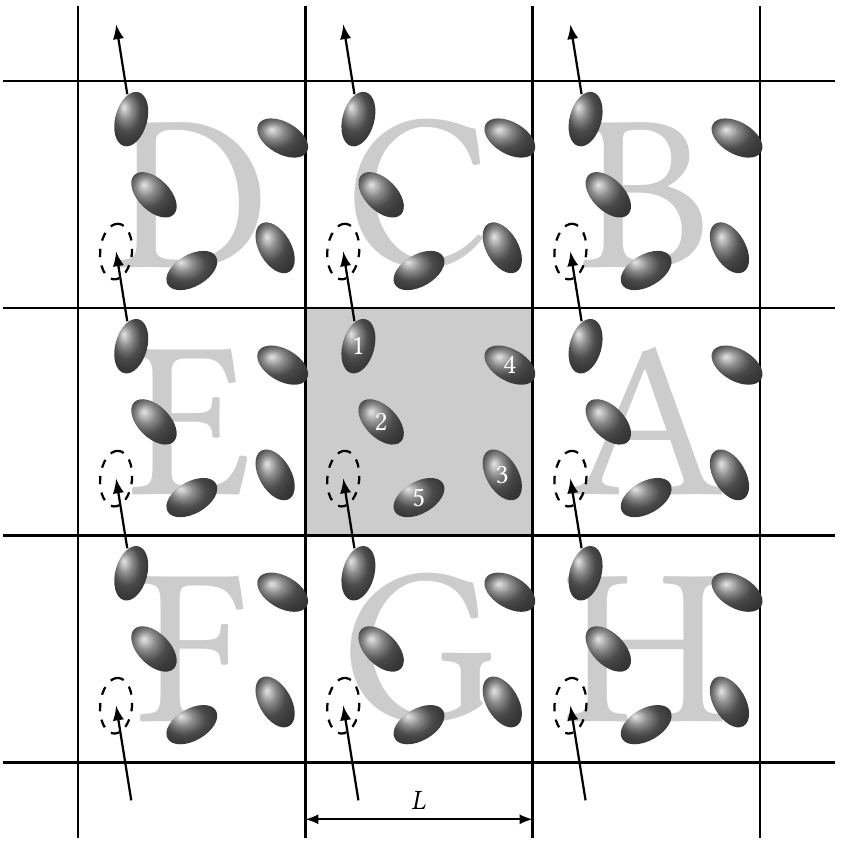
\includegraphics[width=.7\textwidth,keepaspectratio=true]{PBC.png}
    \caption{Un sistema periódico bidimensional \cite{Allen2017}}
    \label{fig:PBC}
\end{figure}

Las condiciones de frontera periódicas simulan la presencia de un bulto. El problema de usar estas condiciones es que al calcular el potencial o la fuerza entre pares se podría tomar en cuenta la fuerza de si misma, esto esta prohibido por la ecuación (\ref{hamiltoniano}).

Para evitar este problema, truncamos el radio de los potenciales que sean menor o igual que la mitad de la longitud del cubo:

\begin{equation}\label{MIC}
    U(\mathbf{r}_{ij}) =
    \begin{cases} 
    U(\mathbf{r}_{ij}),& \text{si } r_c\leq L/2\\
    0,& \text{si } r_c\geq L/2
    \end{cases}
\end{equation}\\

\section{Termostato de Nose-Hoover}

El termostato de Nosé-Hoover es el mas cercano a un verdadero ensamble canónico, Nosé y Hoover extendieron el hamiltoniano del sistema introduciendo un baño térmico y un término de fricción a las ecuaciones de movimiento. La fricción es proporcional al producto de la velocidad de cada partícula y un parámetro de fricción $\xi$(esta es una cantidad dinámica con su propio momento $p_\xi$). Las ecuaciones de movimiento son reemplazadas por \cite{evans1985} \cite{gromacsdoc}:\\

\begin{equation} \label{NHmotion}
    \frac{d^2\mathbf{r}_i}{dt^2} = \frac{\mathbf{F}_i}{m_i}-\frac{p_\xi}{Q}\frac{d\mathbf{r}_i}{dt}
\end{equation}\\

donde la ecuación de movimiento para el parámetro $\xi$ del baño térmico es:\\

\begin{equation}
    \frac{dp_\xi}{dt}=(T-T_0),\quad T_0\ es\ la\ temperatura\ de\ referencia
\end{equation}\\

La cantidad conservada para las ecuaciones de Nose-Hoover es:\\

\begin{equation} \label{conservedNoseHoover}
    \mathcal{H} = \sum_{i=1}^{N}\frac{\mathbf{p}_i^2}{2m_i} + U(\mathbf{r}_1,...,\mathbf{r}_N)+\frac{p_\xi^2}{2Q} + N_fKT\xi
\end{equation}\\

\begin{equation*} \label{taut}
    \text{donde }Q=\frac{\tau_T^2 T_0}{4\pi^2} \text{ y $N_f$ es el número de grados de libertad del sistema}
\end{equation*}\\

El termostato de Nose-Hoover permite una relajación oscilatoria a la temperatura de referencia por lo que tarda mas tiempo que otros termostatos en llegar a la temperatura de referencia.\\

\section{Barostato de Parrinello-Rahman}\textcolor{red}{checar con detenimiento y pensar si separar en barostato y termostato, unirlos con el algoritmo MTK}

Este barostato nos da un verdadero ensamble NPT. Con el barostato los vectores de la caja estan representados por $\mathbf{b}$ y obedecen la ecuación de movimiento matricial\cite{gromacsdoc} \cite{simone1993}:\\

\begin{equation} \label{parrrahman}
    \frac{d\mathbf{b}^2}{dt^2}=V\mathbf{W}^{-1}\mathbf{b'}^{-1}(\mathbf{P}-\mathbf{P}_{ref})
\end{equation}\\

El volumen de la caja es $V$, $\mathbf{W}$ es la matriz de parámetros que determina la fuerza de acoplamiento y las matrices $\mathbf{P},\mathbf{P}_{ref}$ es la presión instantánea y la presión de referencia respectivamente. Este barostato comunmente se usa en combinación con el termostato Nose-Hoover. Asi las ecuaciones de movimiento y la cantidad conservada $\mathcal{H}$ es \cite{gromacsdoc}:

\begin{equation} \label{NHPRmotionr}
    \frac{d^2\mathbf{r}_i}{dt^2} = \frac{\mathbf{F}_i}{m_i}-\frac{p_\xi}{Q}\frac{d\mathbf{r}_i}{dt} + \frac{\mathbf{r}_i}{dV}\left(\ddot{V}-\frac{2\dot{V}}{V}\right)
\end{equation}
\begin{equation} \label{NHPRmotionV}
    \frac{d^2 V}{dt^2} = \frac{\dot{\xi}\dot{V}}{\xi} + \xi^2\mathbf{W}^{-1}(\mathbf{P}-\mathbf{P}_{ref})
\end{equation}
\begin{equation} \label{conservedNoseHooverParrRahm}
    \mathcal{H} = \sum_{i=1}^{N}\frac{\mathbf{p}_i^2}{2m_i} + U(\mathbf{r}_1,...,\mathbf{r}_N)+\frac{p_\xi^2}{2Q} + N_fKT\xi + \sum_i P_{ii}V + \sum_{i,j}\frac{1}{2}W_{ij}\left(\frac{db_{ij}}{dt}\right)^2
\end{equation}\\

con $\mathbf{W}^{-1}_{ij}=\frac{4\pi^2 \beta_{ij}}{3\tau_{p}^2 L}$ y L la longitud del cubo

\section{Campos de fuerzas}

Los campos de fuerzas en una simulación es la energía potencial entre pares que obedecerá el sistema cuando se realicen cálculos de fuerzas. Existen muchos tipos de energías potenciales de interacción entre pares utilizados en la dinámica molecular. Este proceso es parte de la modelación del sistema y es importante para reproducir resultados experimentales. Comúnmente un campo de fuerzas tipo I es como el siguiente:

\begin{align*}\label{FF}
    U_{conf} &= \sum_{enlaces}K_r\left(r-r_0\right)^2 + \sum_{angulos}K_{\theta}\left(\theta-\theta_0\right)^2 \\
             &+ \sum_{diedros}K_{\phi}\left[1-cos(n\phi-\delta)\right] \\
             &+ \sum_{diedros\ impropios}K_{\omega}\left(\omega-\omega_0\right)^2 + \sum_{cargas}\left(\frac{q_i q_j}{4\pi \epsilon r^2_{ij}}\right) \\
             &+ \sum_{VdW} 4 \epsilon_{ij}\left[\left(\frac{\sigma_{ij}}{r_{ij}}\right)^{12}-\left(\frac{\sigma_{ij}}{r_{ij}}\right)^{6}\right]    
\end{align*}

La siguiente tabla \ref{FFallen} muestra otros campos de fuerzas:

\begin{table}[h!]
    \centering
    \begin{tabular}{l c l}
    \hline
    Campo de Fuerza & Clase & Dominio \\
    \hline
    OOPLS & I & péptidos y pequeños orgánicos \\
    CHARM27 & I & ADN, ARN y lípidos \\
    GAFF & I & pequeños orgánicos y diseño de drogas \\
    GROMOS ffG45a3 & I & lípidos y micelas\\
    clayFF & II & minerales hidratados \\
    AMBER ff02 & III & átomos polarizables \\
    AMOEBA & III & multipolos polarizables y multipolos distribuidos \\
    MARTINI & III & modelos de grano grueso, proteinas, lípidos y polímeros \\
    \hline
    \end{tabular}
    \caption{Ejemplo de campo de fuerzas, dominios de aplicación y clases\cite{Allen2017}}
    \label{FFallen}
\end{table}

\begin{itemize}
    \item Tipo I: son potenciales parametrizados para cada tipo de átomo en el sistema.
    \item Tipo II: potenciales parametrizados para todos los átomos incluyendo términos cúbicos en enlaces y otros.
    \item Tipo III: potenciales parametrizados para todos los átomos extendiendo los cálculos electrostáticos para incluir polarización. Estos también incluyen a los campos de grano grueso.
\end{itemize}

